\begin{enumerate}
\item Let $A = \{1,2,4,5\}$, $B=\{2,3,4,6\}$, and $C=\{1,2,3,4\}$.  Place each of the elements $1, \ldots , 6$ in the appropriate regions of a three-set Venn diagram.

\centerline{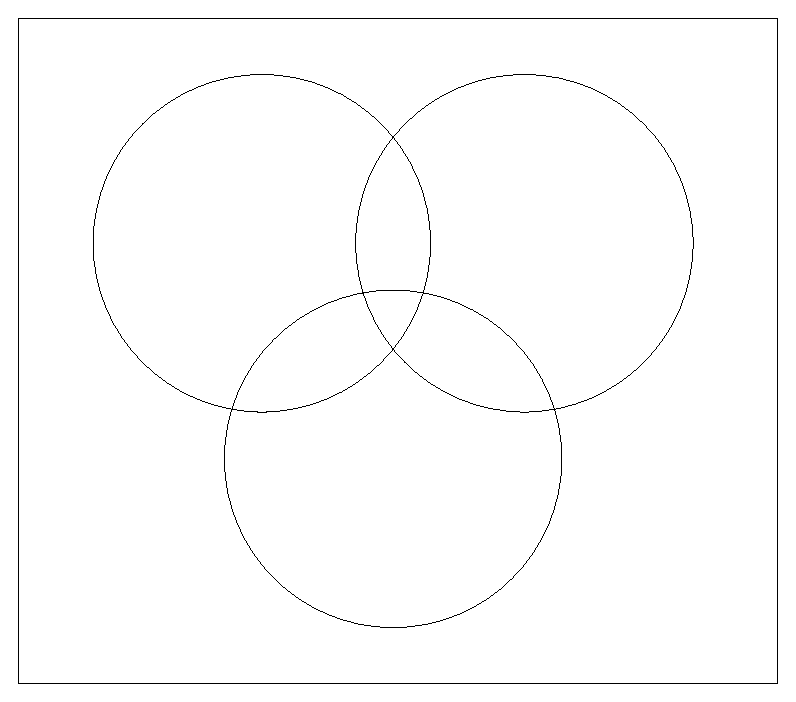
\includegraphics[scale=.75]{figures/3set_Venn}}

\hint{The center region contains $2$ and $4$.}

\item Prove or disprove:

\[ ( A \cap C \; \subseteq \; B \cap C ) \quad \implies \quad A \; \subseteq B \]

\hint{What will be the implications of the region $A \cap \overline{B} \cap \overline{C}$ being non-empty?}

\newpage

\item  Venn diagrams are usually made using simple closed curves 
with no further restrictions.  Try creating Venn diagrams for 3, 4 and
5 sets (in general position) using rectangular simple closed curves.

\hint{I found it easier to experiment by making my drawings on graph paper.  I never did  
manage to draw the $5$ set Venn diagram with just rectangles\ldots probably just a lack of persistence.}

\wbvfill

\workbookpagebreak

\item  We call a curve \emph{rectilinear} if it is made
of line segments that meet at right angles.  If you have ever
played with an Etch-a-Sketch you'll know what we mean by the term 
``rectilinear.''  The following example of a rectilinear curve may
also help to clarify this notion.

\centerline{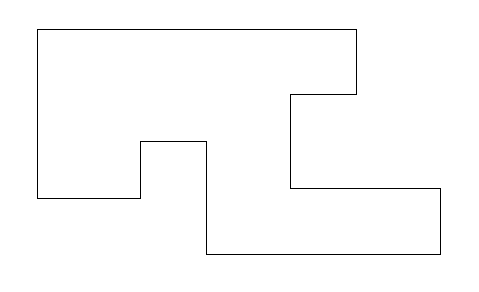
\includegraphics{figures/rectilinear}}

Use rectilinear
simple closed curves to create a Venn diagram for 5 sets.

\hint{Of course, rectangles are rectilinear, so one could use the solution from the previous
problem (if, unlike me, you were persistant enough to find it).  Otherwise, 
start with the $4$ set diagram made with rectangles and use your $5$th (rectilinear) curve to split
each region into $2$ -- don't forget to split the region on the outside too.}

\wbvfill

\workbookpagebreak
\hintspagebreak

\item  Argue as to why rectilinear curves will suffice to build
any Venn diagram.

\hint{Fortunately the instructions don't say to {\em prove} that rectilinear curves will always
suffice, so we can be less rigorous.  Try to argue as to why it will alway be possible to add one more rectilinear curve to an existing Venn diagram and split every region into two.

One might also argue that any continuous curve can be approximated using rectilinear curves.  So if a Venn diagram can be constructed using continuous curves we can also get the job done with rectilinear curves.}

\wbvfill



\item  Find the disjunctive normal form of $A \cap (B \cup C)$.

\hint{ $ (A \cap B \cap \overline{C}) \cup (A \cap \overline{B} \cap C) $ }

\wbvfill

\workbookpagebreak

\item  Find the disjunctive normal form of $(A \triangle B) \triangle C$

\hint{It is $(A \cap \overline{B} \cap \overline{C}) \cup (\overline{A} \cap B \cap \overline{C}) \cup (\overline{A} \cap \overline{B} \cap C)$.  Now find the disjunctive normal form of 
$A \triangle (B \triangle C)$.}

\wbvfill

\item The prototypes for the \emph{modus ponens} and \emph{modus tollens}
argument forms are the following:

\begin{tabular}{lcl}
\begin{minipage}{.3\textwidth}All men are mortal. \newline %
Socrates is a man. \newline
Therefore Socrates is mortal.\end{minipage} & \rule{16pt}{0pt} and \rule{16pt}{0pt} & %
 \begin{minipage}{.3\textwidth}All men are mortal. \newline %
Zeus is not mortal. \newline
Therefore Zeus is not a man.\end{minipage}
\end{tabular}

Illustrate these arguments using Venn diagrams.

\hint{The statement ``All men are mortal'' would be interpreted on a Venn diagram by showing the
set of ``All men'' as being entirely contained within the set of ``mortal beings.''   Socrates is an 
element of the inner set.  Zeus, on the other hand, lies outside of the outer set.}
 
 \wbvfill
 
 \workbookpagebreak
 \hintspagebreak

\item Use Venn diagrams to convince yourself of the validity of
the following containment statement

\[ (A \cap B) \cup (C \cap D) \; \subseteq \; (A \cup C) \cap (B \cup D).\]

Now prove it!
 
\hint{Obviously we'll need one of the $4$-set Venn diagrams.}
 
 \wbvfill
 
 \workbookpagebreak
 
\item Use Venn diagrams to show that the following set equivalence is false.

\[ (A \cup B) \cap (C \cup D) \; = \; (A \cup C) \cap (B \cup D) \]

\hint{After constructing Venn diagrams for both sets you should be able to see that there
are $4$ regions where they differ.  One is $A \cap B \cap \overline{C} \cap \overline{D}$.
What are the other three?}

\wbvfill
 
 \workbookpagebreak
 
\end{enumerate}



%% Emacs customization
%% 
%% Local Variables: ***
%% TeX-master: "GIAM-hw.tex" ***
%% comment-column:0 ***
%% comment-start: "%% "  ***
%% comment-end:"***" ***
%% End: ***

